
\documentclass{article}

\usepackage{natbib}
\usepackage{graphics}
\usepackage{amsmath}
\usepackage{indentfirst}
\usepackage[utf8]{inputenc}
\usepackage{color}
\usepackage{hyperref}

% \VignetteIndexEntry{msgbsR_Example}
%\VignetteEngine{knitr::knitr}

\usepackage{Sweave}
\begin{document}
\Sconcordance{concordance:msgbsR_Vignette.tex:msgbsR_Vignette.Rnw:%
1 13 1 1 0 22 1 1 2 1 0 1 1 1 2 1 1 1 2 3 0 1 2 8 1 1 2 1 0 1 1 1 2 5 1 %
3 0 1 2 4 1 1 2 1 0 1 2 4 0 1 2 2 1 1 2 1 0 1 2 8 0 1 2 3 1 1 2 4 0 1 2 %
7 1 1 2 1 0 2 1 3 0 1 2 5 1 2 2 12 1 1 5 7 0 1 2 7 1 1 2 4 0 1 2 1 1 1 %
2 1 0 3 1 3 0 1 2 1 1 1 3 6 0 1 3 1 1 1 2 4 0 1 2 3 1 2 3 10 1 2 2 11 1 %
1 2 1 0 1 2 7 0 1 1 11 0 1 2 2 1 1 2 70 0 1 2 5 1}


\title{msgbsR: an R package to analyse methylation sensitive genotyping by sequencing (MS-GBS) data}
\author{Benjamin Mayne}
\maketitle

\tableofcontents

\clearpage

\section{Introduction}

Current data analysis tools do not fulfil all experimental designs. For example, GBS experiments using methylation sensitive restriction enzymes (REs), which is also known as methylation sensitive genotyping by sequencing (MS-GBS), is an effective method to identify differentially methylated sites that may not be accessible in other technologies such as microarrays and methyl capture sequencing. However, current data analysis tools do not satisfy the requirements for these types of experimental designs.

Here we present msgbsR, an R package for data analysis of MS-GBS experiments. Read counts and cut sites from a MS-GBS experiment can be read directly into the R environment from a sorted and indexed BAM file(s).

\section{Reading data into R}

The analysis with the msgbsR pipeline begins with a directory which contains sorted and indexed BAM file(s). msgbsR contains an example data set containing 6 samples from a MS-GBS experiment using the restriction enzyme MspI. In this example the 6 samples are from the prostate of a rat and have be truncated for chromosome 20. 3 of the samples were fed a control diet and the other 3 were fed an experimental high fat diet.

To read in the data directly into the R environment can be done using the rawCounts() function, which requires the directory path to where the sorted and indexed files are located and the desired number of threads to be run (Default = 1).

\begin{Schunk}
\begin{Sinput}
> library(msgbsR)
> library(ggplot2)
> my_path <- system.file("extdata", "Control_1.bam", package = 'msgbsR')
> my_path <- gsub('Control_1.bam', '', my_path)
> datCounts <- rawCounts(bamFilepath = my_path, threads = 1)
\end{Sinput}
\end{Schunk}

The result is a data frame object containing a table of read counts. The columns are samples and the rows contain the location of each unique cut sites. Each cut site has been given a unique ID (chromosome:strand:position).

\section{Confirmation of correct cut sites}

After the table of read counts has been generated into the R environment, the next step is to confirm that the cut sites were the correctly generated sites. In this example, the restriction enzyme that has been used is MspI which recognizes a 4bp sequence (CCGG).

The first step is to extract the location of the cut sites from datCounts and adjust the cut sites such that the region will cover the recognition sequence of MspI.

\begin{Schunk}
\begin{Sinput}
> x <- data.frame(row.names(datCounts))
> x <- data.frame(t(data.frame(strsplit(x=as.character(x[,1]), split=':'))))
> x[,2] <- x[,3]
> x <- as.matrix(x)
> row.names(x) <- NULL
> x[,3] <- as.numeric(x[,3]) +2
> x[,2] <- as.numeric(x[,2]) -1
> x <- as.matrix(x)
\end{Sinput}
\end{Schunk}

The object x is a matrix that contains the chromosome ID, the start and end position of the MspI sequence length around the cut sites. These cut sites can now be checked if the sequence matches the MspI sequence.

msgbsR offer two approaches to checking the cut sites. The first approach is to use a BSgenome which can be obtained from Bioconductor. In this example, BSgenome.Rnorvegicus.UCSC.rn6 will be used.

\begin{Schunk}
\begin{Sinput}
> library(BSgenome.Rnorvegicus.UCSC.rn6)
> correctCuts <- checkCuts(cutSites = x, cutIDs = row.names(datCounts),
+                          BSgenome = Rnorvegicus, seq = 'CCGG')
\end{Sinput}
\end{Schunk}

If a BSgenome is unavailable, another option to checking the cut sites is to use a fasta file. msgbsR comes with the fasta file for chromosome 20 from UCSC rn6. To use the checkCuts function with a fasta file simply leave the BSgenome input as blank (NULL) and input the path to the fasta file location. An example of this is shown below.

\begin{Schunk}
\begin{Sinput}
> chr20 <- system.file("extdata", "chr20.fa.gz", package = 'msgbsR')
> correctCuts <- checkCuts(cutSites = x, cutIDs = row.names(datCounts),
+                          fastaPath = chr20, seq = 'CCGG')
\end{Sinput}
\begin{Soutput}
[1] "Uncompressing fasta file"
[1] "Compressing fasta file"
\end{Soutput}
\end{Schunk}

The correctCuts data object now contains the correct cut site locations of MspI that were generated from this experiment.

The incorrect MspI cut sites can be filtered out of datCounts:
\begin{Schunk}
\begin{Sinput}
> datCounts <- datCounts[match(correctCuts, row.names(datCounts)), ]
\end{Sinput}
\end{Schunk}

datCounts now contains the correct cut sites and can now be used in downstream analyses.

\section{Visualization of read counts}

Before any further downstream analyses with the table of read counts, the user may want to filter out samples that did not generate a sufficient number of read counts or cut sites. The msgbsR package contains a function which plots the total number of read counts against the total number of cut sites produced per sample.

To visualize the total number of read counts against the total number of cut sites produced per sample:
\begin{Schunk}
\begin{Sinput}
> y <- data.frame(c(rep('Control', 3), rep('Fat Diet', 3)))
> colnames(y) <- 'Group'
> plotCounts(countMatrix = datCounts, condition1 = y$Group)
\end{Sinput}
\end{Schunk}

This function generates a plot (Figure 1) where the x axis and y axis represents the total number of reads and the total number of cut sites produced for each sample respectively.

\setkeys{Gin}{width=1\linewidth}
\begin{figure}
\begin{center}
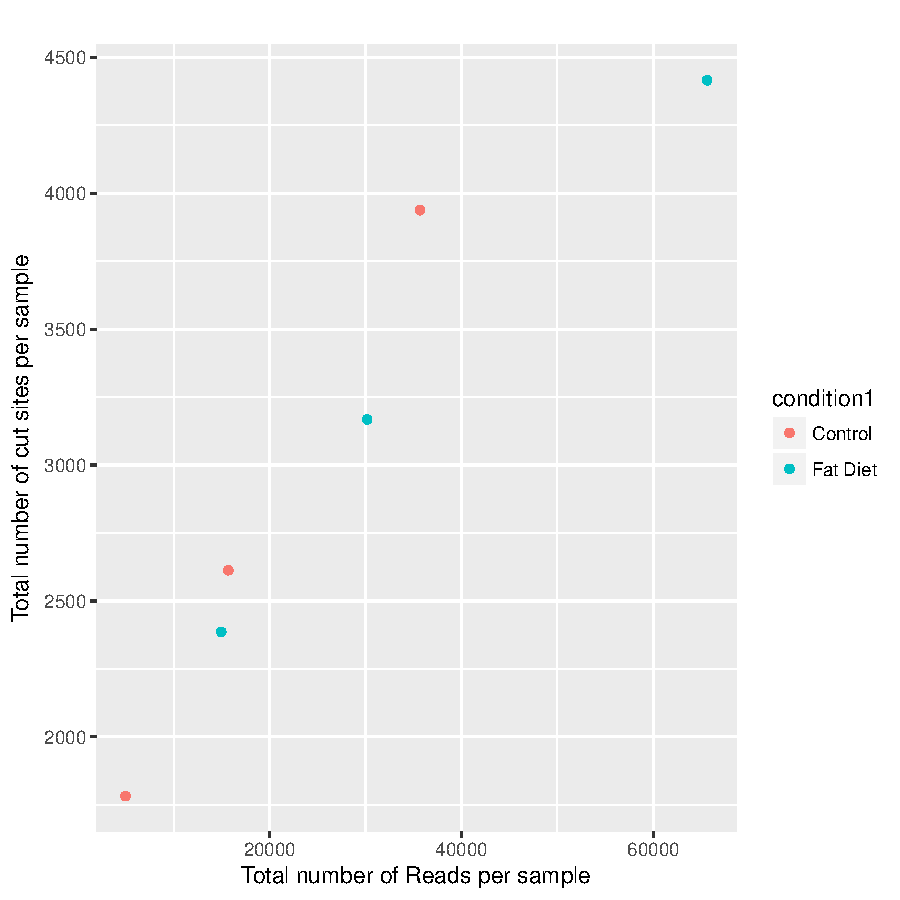
\includegraphics{msgbsR_Vignette-fig1}
\end{center}
\caption{The distribution of the total number of reads and cut sites produced by each sample.}
\label{fig:fig1}
\end{figure}

\clearpage


\section{Differential methylation analysis}

msgbsR utilizes edgeR in order to determine which cut sites are differentially methylated between groups. Since MS-GBS experiments can have multiple groups or conditions msgbsR offers a wrapper function of edgeR (Zhou et al., 2014) tools to automate differential methylation analyses.

To determine which cut sites are differentiallly methylated between groups:
\begin{Schunk}
\begin{Sinput}
> top <- diffMeth(countMatrix = datCounts, pd = y, cateogory = 'Group',
+                 condition1 = 'Control', condition2 = 'Fat Diet',
+                 block = NULL,
+                 cpmThreshold = 1, thresholdSamples = 1)
\end{Sinput}
\end{Schunk}

The top object now contains a data frame of the cut sites that had a CPM > 1 in at least 1 sample and which cut sites are differentially methylated between the two groups.

\section{Visualization of cut site locations}

The msgbsR package contains 2 functions to allow visualization of the location of the cut sites. Given the lengths of the chromosomes the cut sites can be visualized in a circos plot (Figure 2) or a karyogram (Figure 3).

Firstly, define the length of the chromosome.
\begin{Schunk}
\begin{Sinput}
> chr20 <- matrix(c('chr20', '56205956'), nrow = 1, ncol = 2)
\end{Sinput}
\end{Schunk}

Extract the top 100 most differentially methylated cut sites.
\begin{Schunk}
\begin{Sinput}
> z <- top$cut_site[which(top$PValue < 0.05)]
> z <- data.frame(t(data.frame(strsplit(x=as.character(z), split=':'))))
> z <- as.matrix(z)
> row.names(z) <- NULL
\end{Sinput}
\end{Schunk}

To generate a circos plot:
\begin{Schunk}
\begin{Sinput}
> plotCircos(cutSites = z[,c(1,3,3)], genome = chr20,
+            cutSite.colour = 'red', genome.colour = 'blue')
> 
\end{Sinput}
\end{Schunk}

To generate a karogram plot:
\begin{Schunk}
\begin{Sinput}
> plotChr(cutSites = z[,c(1,3,3)], genome = chr20)
\end{Sinput}
\end{Schunk}

\setkeys{Gin}{width=1\linewidth}
\begin{figure}
\begin{center}
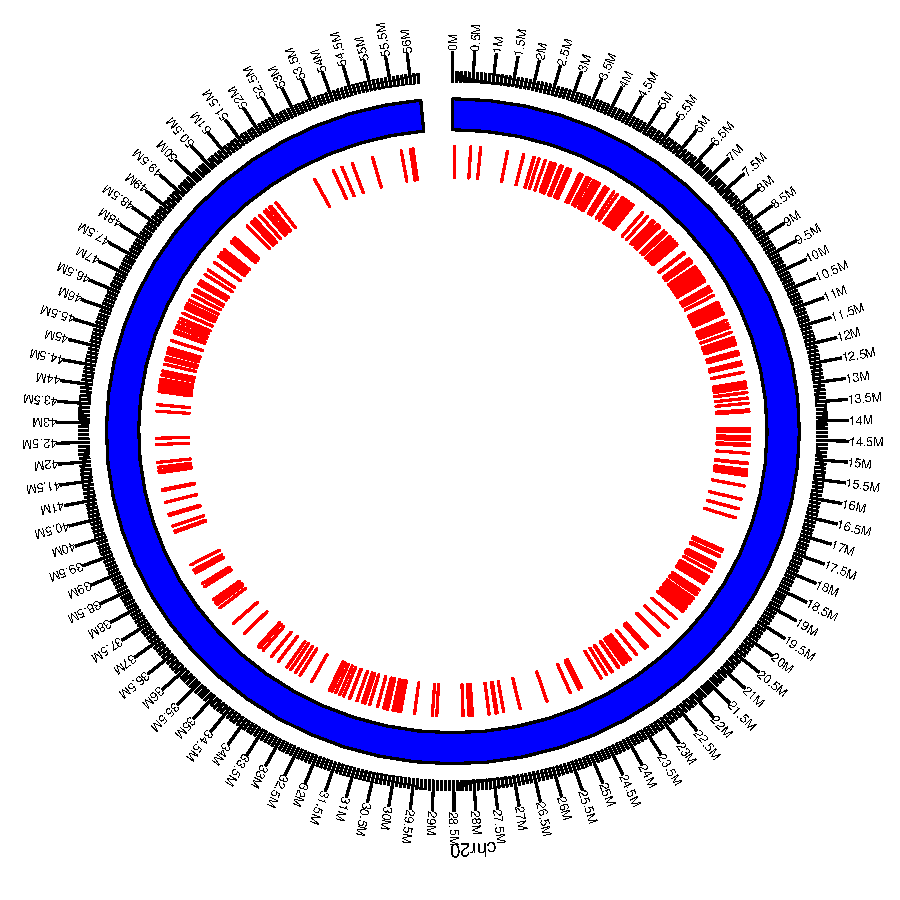
\includegraphics{msgbsR_Vignette-fig2}
\end{center}
\caption{A circos plot of chromosome 20 representing cut sites defined by the user.}
\label{fig:fig2}
\end{figure}

\clearpage


\setkeys{Gin}{width=1\linewidth}
\begin{figure}
\begin{center}
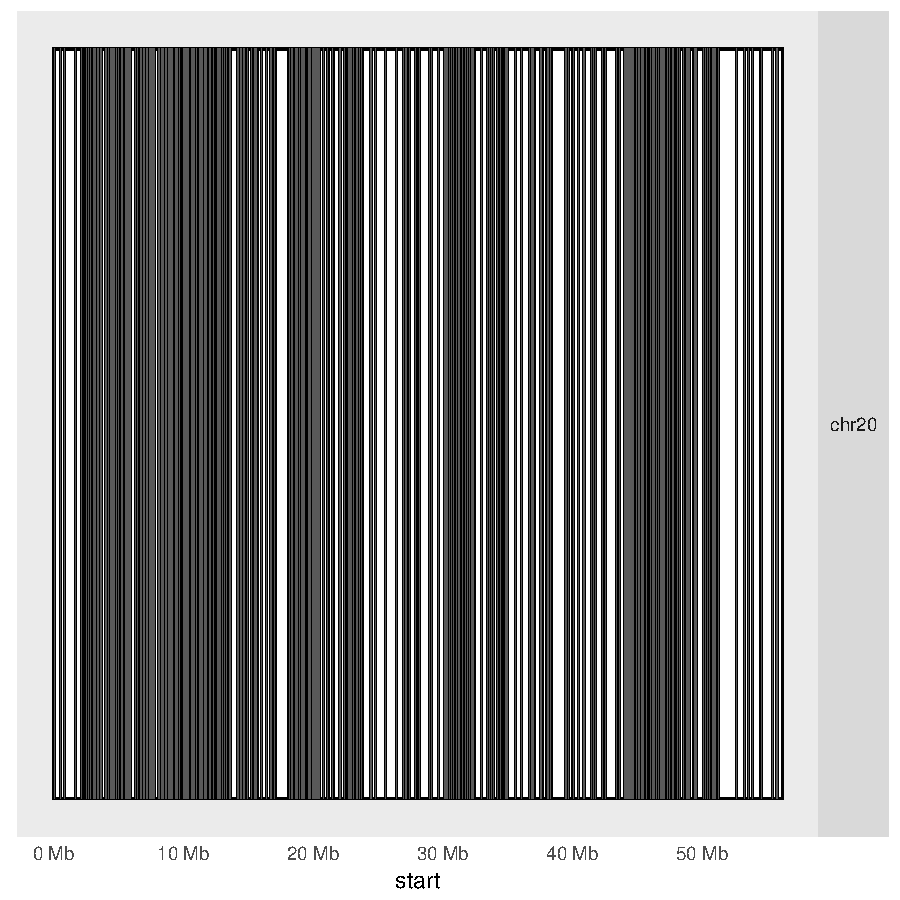
\includegraphics{msgbsR_Vignette-fig3}
\end{center}
\caption{A karyogram of chromosome 20 showing cut sites defined by the user.}
\label{fig:fig3}
\end{figure}

\clearpage

\section{Annotation}

The msgbsR package can also work with gff3 files to annotate interesting positions such as those that might be differentially methylated. Annotation can be done using the closestFeat() function. To use closestFeat() the user needs to input the path to the gff3 file, the cut sites in the form of a matrix and whether or not the user wants to look at strand specific features.

To annotate interesting cut sites:
\begin{Schunk}
\begin{Sinput}
> mygff <- system.file("extdata", "chr20.gff3", package = 'msgbsR')
> features <- closestFeat(gff = mygff, positions = z,
+                         strand.specific = FALSE)
\end{Sinput}
\begin{Soutput}
[1] "Reading in the gff file"
[1] "Finding closest features"
\end{Soutput}
\begin{Sinput}
> features[1:5,1:5]
\end{Sinput}
\begin{Soutput}
  Distance seqname feature    start      end
1    31268   chr20    exon 48923592 48924162
2  -655854   chr20    mRNA 37585713 37589018
3    12066   chr20    exon 48923592 48924162
4   115542   chr20    exon 40800231 40800842
5     3751   chr20    exon  8876254  8876421
\end{Soutput}
\end{Schunk}

\section{Session Information}
This analysis was conducted on:
\begin{Schunk}
\begin{Sinput}
> sessionInfo()
\end{Sinput}
\begin{Soutput}
R version 3.3.1 (2016-06-21)
Platform: x86_64-w64-mingw32/x64 (64-bit)
Running under: Windows 10 x64 (build 10586)

locale:
[1] LC_COLLATE=English_Australia.1252  LC_CTYPE=English_Australia.1252   
[3] LC_MONETARY=English_Australia.1252 LC_NUMERIC=C                      
[5] LC_TIME=English_Australia.1252    

attached base packages:
[1] stats4    parallel  stats     graphics  grDevices utils     datasets 
[8] methods   base     

other attached packages:
 [1] BSgenome.Rnorvegicus.UCSC.rn6_1.4.1 BSgenome_1.40.1                    
 [3] rtracklayer_1.32.2                  Biostrings_2.40.2                  
 [5] XVector_0.12.1                      GenomicRanges_1.24.3               
 [7] GenomeInfoDb_1.8.7                  IRanges_2.6.1                      
 [9] S4Vectors_0.10.3                    BiocGenerics_0.18.0                
[11] ggplot2_2.2.0                       msgbsR_0.99.5                      

loaded via a namespace (and not attached):
 [1] Biobase_2.32.0                httr_1.2.1                   
 [3] edgeR_3.14.0                  AnnotationHub_2.4.2          
 [5] splines_3.3.1                 R.utils_2.5.0                
 [7] genomeIntervals_1.28.0        Formula_1.2-1                
 [9] shiny_0.13.2                  assertthat_0.1               
[11] interactiveDisplayBase_1.10.3 latticeExtra_0.6-28          
[13] RBGL_1.48.1                   Rsamtools_1.24.0             
[15] RSQLite_1.0.0                 lattice_0.20-33              
[17] biovizBase_1.20.0             limma_3.28.21                
[19] digest_0.6.10                 chron_2.3-47                 
[21] RColorBrewer_1.1-2            colorspace_1.2-6             
[23] ggbio_1.20.2                  httpuv_1.3.3                 
[25] htmltools_0.3.5               Matrix_1.2-6                 
[27] R.oo_1.20.0                   plyr_1.8.4                   
[29] OrganismDbi_1.14.1            XML_3.98-1.4                 
[31] ShortRead_1.30.0              biomaRt_2.28.0               
[33] genefilter_1.54.2             zlibbioc_1.18.0              
[35] xtable_1.8-2                  scales_0.4.1                 
[37] intervals_0.15.1              BiocParallel_1.6.6           
[39] LSD_3.0                       tibble_1.2                   
[41] annotate_1.50.1               SummarizedExperiment_1.2.3   
[43] GenomicFeatures_1.24.5        easyRNASeq_2.8.2             
[45] nnet_7.3-12                   lazyeval_0.2.0               
[47] mime_0.5                      survival_2.39-4              
[49] magrittr_1.5                  GGally_1.2.0                 
[51] R.methodsS3_1.7.1             hwriter_1.3.2                
[53] foreign_0.8-66                graph_1.50.0                 
[55] BiocInstaller_1.22.3          tools_3.3.1                  
[57] data.table_1.9.6              stringr_1.1.0                
[59] munsell_0.4.3                 locfit_1.5-9.1               
[61] cluster_2.0.4                 AnnotationDbi_1.34.4         
[63] ensembldb_1.4.7               DESeq_1.24.0                 
[65] grid_3.3.1                    RCurl_1.95-4.8               
[67] dichromat_2.0-0               VariantAnnotation_1.18.7     
[69] labeling_0.3                  bitops_1.0-6                 
[71] gtable_0.2.0                  DBI_0.5                      
[73] reshape_0.8.5                 reshape2_1.4.1               
[75] R6_2.1.3                      GenomicAlignments_1.8.4      
[77] gridExtra_2.2.1               Hmisc_3.17-4                 
[79] stringi_1.1.1                 Rcpp_0.12.6                  
[81] geneplotter_1.50.0            rpart_4.1-10                 
[83] acepack_1.3-3.3              
\end{Soutput}
\end{Schunk}

\section{References}
\paragraph{} \hspace{0pt} \\
Zhou X, Lindsay H, Robinson MD (2014). Robustly detecting differential expression in RNA sequencing data using observation weights. Nucleic Acids Research, 42(11), e91.

\end{document}
